\section{Wandler}

\subsection{Kennlinien\hartl{432}}
\begin{tabular}{|p{5.5cm}|c|c|} %>{\bfseries}p{0.25\textwidth}|c|c|}
	\hline
	& \textbf{ADC} & \textbf{DAC} 
	\\ \hline
	\textbf{Kennlinien idealer Wandler}
	& \parbox[c][6cm]{0.31\textwidth}{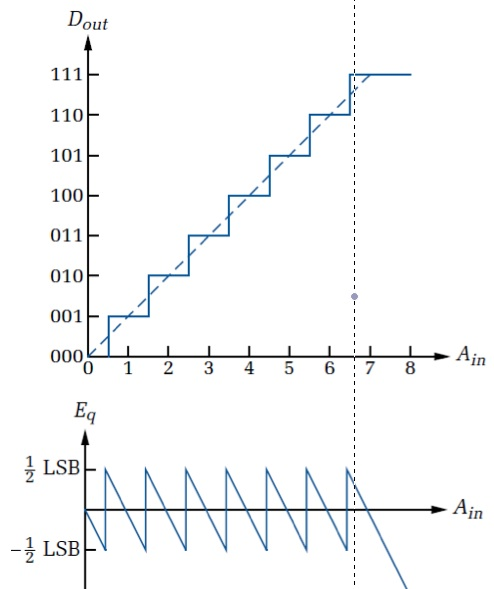
\includegraphics[height=5cm]{./images/idealerADC.jpg}}
	& \parbox[c]{0.31\textwidth}{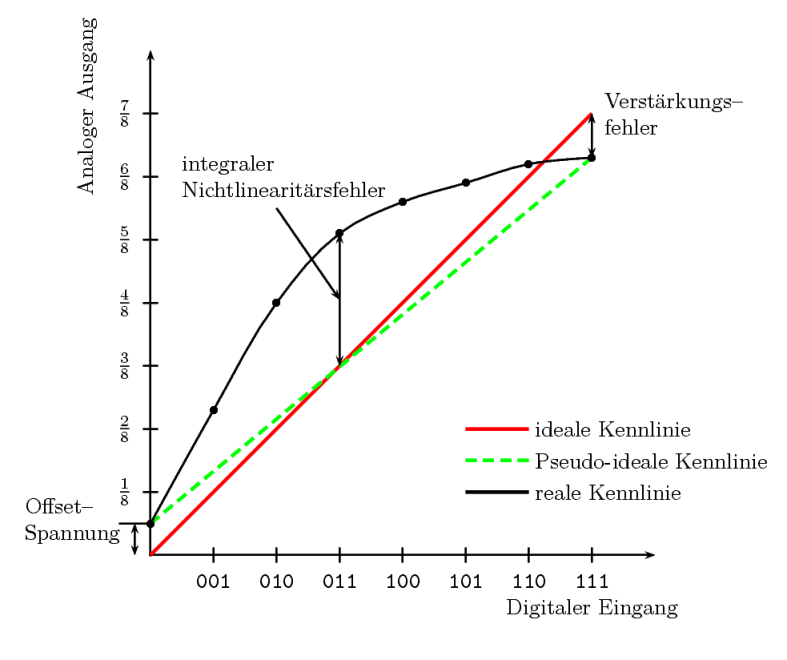
\includegraphics[width=0.3\textwidth]{./images/idealerDAC.png}}
	\\ \hline
	\textbf{Quantisierungsintervall}
	& $q = \frac{A_{max}}{2^N} = \frac{V_{Refp}-V_{Refn}}{2^N}$
	& $q = \frac{A_{Ref}}{2^N} = \frac{V_{Refp}-V_{Refn}}{2^N} = 1LSB $
	\\ \hline
	\textbf{Quantisierungsfehler}
	& $ -\frac{q}{2}\leq E_{q}<+\frac{q}{2} $
	&
	\\ \hline 
	\textbf{Ausgangsgrösse}
	& $D_{out} = \frac{V_{in} - V_{Refn}}{q} = \frac{V_{in} - V_{Refn}}{V_{Refp}-V_{Refn}} \cdot 2^{N}$
	& $V_{out} = D_{in}\cdot q + V_{Refn}= D_{in}\cdot(\frac{A_{Ref}}{2^N}) + V_{Refn}$
	\\ \hline
	\textbf{Offset-Fehler \hartl{434}}
	& 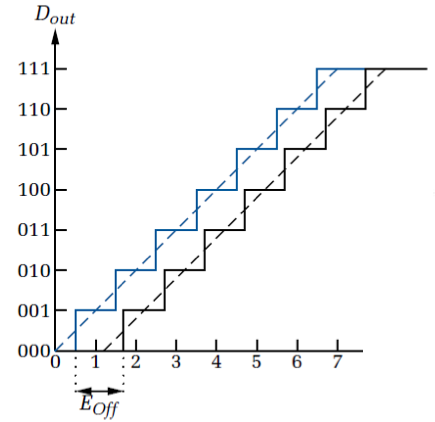
\includegraphics[height=3cm, trim=0cm 0cm 6.2cm 6.5cm, clip=true, valign=t]{./images/EoffADC.png}
	& 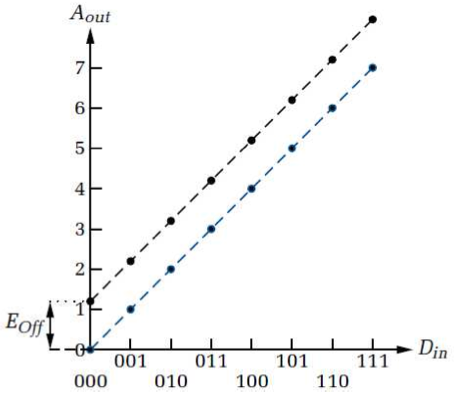
\includegraphics[height=3cm, trim=0cm 0cm 6cm 6.5cm, clip=true, valign=t]{./images/EoffDAC.png}
	\\ \hline
	\textbf{Verstärkungsfehler \hartl{436}}
	& 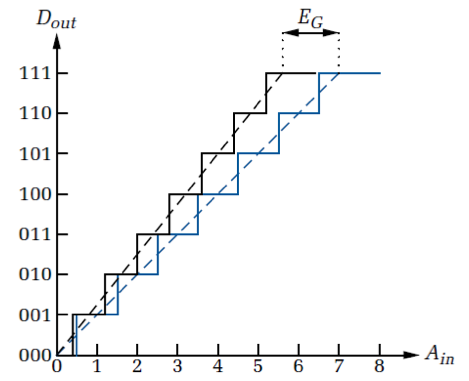
\includegraphics[height=3cm, valign=t]{./images/verstaerkungsfehlerADC.png} 
    & 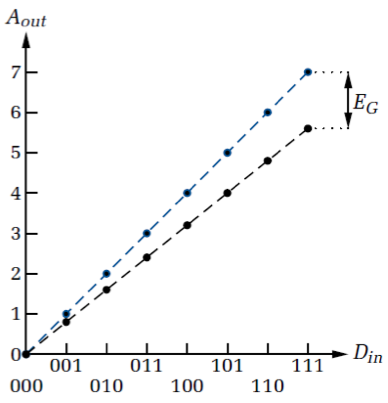
\includegraphics[height=3cm, valign=t]{./images/verstaerkungsfehlerDAC.png}
	\\ \hline
	\textbf{Differentielle Nichtlinearität DNL \hartl{437}} \newline \newline
  $DNL_n$ = (Spannungsinkrement bei einem Eingangsschritt von $n-1$ nach $n$) -
  (ideales Spannungsinkrement q) in LSB
	& 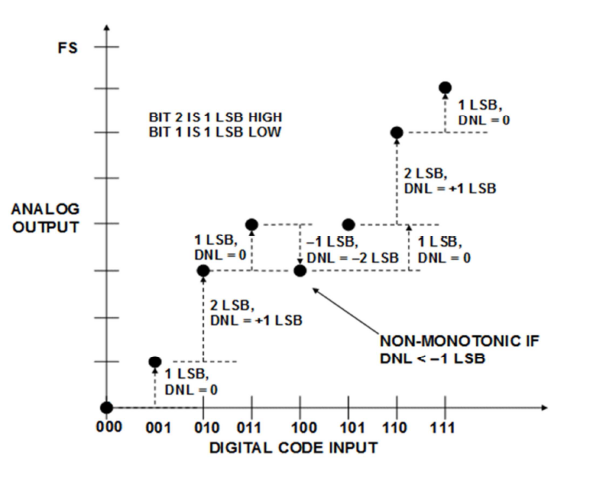
\includegraphics[height=3cm, valign=t]{./images/DNL_ges.png}
	& 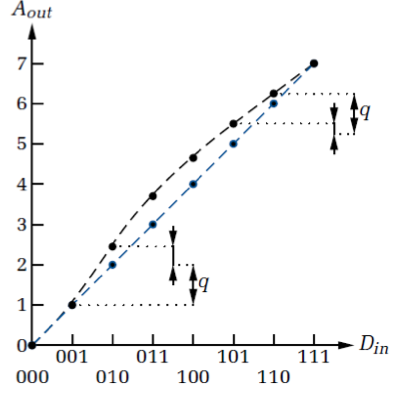
\includegraphics[height=3cm, valign=t]{./images/DNL_DAC.png}
	\\ \hline
	\textbf{Integrale Nichtlinearität INL \hartl{439}} \newline \newline
  Die INL bezeichnet die max. Abweichung der Ausgangskurve von der Idealen Gerade.
	& 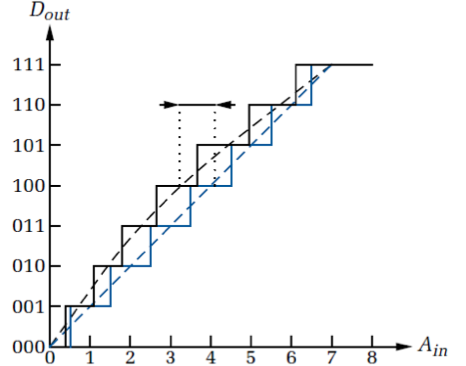
\includegraphics[height=3.5cm, valign=t]{./images/INL_ADC.png}
	& 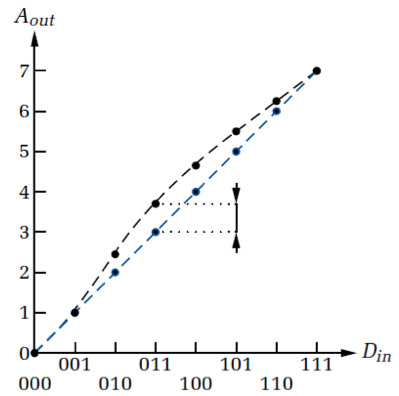
\includegraphics[height=4cm, valign=t]{./images/INL_DAC.png}
	\\ \hline
\end{tabular}
\subsection{Eigenschaften und Fehler bei dynamischen Signalen\hartl{442}}

\begin{tabular}{l p{11cm}}
  \textbf{SFDR (Spurios Free Dynamic Range):} &
  Abstand von der Grundwelle zum höchsten Peak der Harmonischen. \\
  \textbf{Verzögerungszeit (Settling Time):} &
  Zeit vom Anlegen des Signals bis das Signal innerhalb vom Fehlerband ist und nicht mehr hinaus geht.
\end{tabular}

\subsubsection{Aperturfehler\hartl{442}} 
Bei periodischer Abtastung eines Signals ist immer ein gewisse zeitliche
Unsicherheit im Abtastzeitpunkt (Aperturunsicherheit) gegeben. Ist der Aperturfehler grösser als der maximal auftretende Quantisierungsfehler ($\frac{1}{2}LSB$) so verschlechtert sich die Auflösung.
\newpage

\subsubsection{Jitterfehler}
\begin{longtable}[c]{ l  l l l }
\begin{minipage}{4cm}

  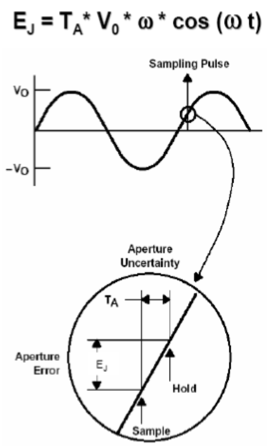
\includegraphics[scale=0.38]{images/aperturfehlercos}

\end{minipage}
&
\begin{minipage}{3cm}

  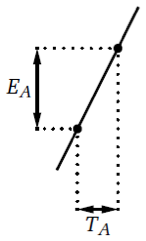
\includegraphics[scale=0.42]{images/aperturfehler}
\end{minipage}
&
\begin{minipage}{5cm}
\begin{gather*}
x(t)=V_0\sin(2\pi ft)\\
\dot{x}(t)=2\pi fV_0\cos(2\pi t)\\
max\mid\dot{x}(t)\mid= 2\pi fV_0 \\
E_{A}=2\pi fV_0T_{A}\\
2V_0=A_{Ref}\\
E_{A}<E_{q}\\
E_{q}=\frac{q}{2}=\frac{A_{Ref}}{2\cdot2^N}\\
E_{A}<\frac{A_{Ref}}{2\cdot2^N}\\
2\pi fV_0T_{A} <\frac{2V_0}{2\cdot2^N}\\
T_{A} < \frac{1}{\pi f2^{N+1}}
\end{gather*}
\end{minipage}

&
\begin{minipage}{5cm}
\begin{tabular}{ll}
$E_{A}$: &Aperturfehler\\
$E_{q}$:&Quantisierungsfehler\\
$T_{A}$:&Zeitfehler\\
$A_{Ref}$:&analoge Referenz\\
N:& N bit Auflösung\\
$V_0$: &Amplitude\\
f: &Frequenz\\
t: &Zeit\\
x(t):&Signal
\end{tabular}


\end{minipage}
\\
\end{longtable}


\subsubsection{Aliasing\hartl{444}}
Aliasing entsteht bei Unterabtastung, d.h wenn das Abtasttheorem verletzt wird.
Es entstehen falsche, nur scheinbar vorhandene Komponenten im zeitdiskreten
Signal.

	\textbf{Abtasttheorem}  $f_{S}>2f_{max}$ $f_{s}$: Abtastfrequenz $f_{max}$:max. Frequenz des Signals


%\subsection{Lineares Modell der Quantisierung\hartl{448}}
%\subsubsection{Signal-Rausch-Verhältnis\hartl{450}}
%\begin{multicols}{2}
%\begin{align*}
%P_{Sig} &= S^2_{Eff} = \frac{S^2}{2} = \frac{(\frac{A_{Ref}}{2})^2}{2} = \frac{A^2_{Ref}}{8}\\
%P^2_{N} &= \frac{q^2}{12} = \frac{(\frac{A_{Ref}}{2^N})}{12} = \frac{A^2_{Ref}}{12\cdot2^{2N}}\\
%SNR		&= \frac{P^2_{S}}{P^2_{N}} = \frac{\frac{A^2_{Ref}}{8}}{\frac{A^2_{Ref}}{12\cdot2^{2N}}} = \frac{12\cdot2^{2N}}{8} = 3\cdot2^{2N-1}\\
%SNR_{dB}&= 10\log(3\cdot2^{2N-1}) = 6.02N+1.76dB\\
%E$ NO $B	&= \frac{SNR_{dB}-1.76}{6.02}
%\end{align*}
%
%\begin{tabular}{ll}
%$P_{Sig}$:&Signalleistung\\
%SNR:&Signal-Rausch-Verhältnis\\
%$SNR_{dB}$:&Signal-Rausch-Verhältnis in dB\\
%ENOB:&Effektive Anzahl Bits\\
%\end{tabular}
%\end{multicols}